\section[加速度]{\makebox[5em][s]{加速度}}\label{sec:01.08}

为了描写速度的变化,我们再引入一个物理量,即所谓加速
度。对于直线运动,若当$t$时刻,质点速度为$v\left(t\right)$,当$t+\Delta t$时
刻,为$v\left(t+\Delta t\right)$,则我们定义从$t$到$t+\Delta t$间隔中质点的平均加
速度为\\~\vspace{-2em}
\begin{equation}\label{eqn:01.08.01}
  \langle a\rangle_{t\rightarrow t+\Delta t} = \frac{v\left(t+\Delta t\right)-v\left(t\right)}{\Delta t}
\end{equation}
它的定义是质点在单位时间中速度的平均变化,单位是$\text{米/秒}^2$。

利用式\eqref{eqn:01.06.02},可以计算自由落体在$t$到$t+\Delta t$间隔中的平
均加速度:\vspace{-1em}
\begin{equation*}
  \begin{aligned}
    \langle a\rangle_{t\rightarrow t+\Delta t} & = \frac{9.8\left(t+\Delta t\right)-9.8t}{\Delta t} \\
                                               & = 9.8\text{米/秒}^2
  \end{aligned}
\end{equation*}
这个结果中不含$t$和$\Delta t$,也就是说,对任何一段时间间隔,自由落
体的平均加速度都是一样的。这种加速度不随时间变化的运动,
称为匀加速运动。自由落体运动是一个典型的匀加速运动。无论
用何种材料作成的物体,它的自由落体加速度总等于$9.8\text{米/秒}^2$。
称此加速度为重力加速度,用$g$表示。

精确测量表明,在地球各处,重力加速度$g$并不都一样,一

\mbox{}

\begin{table}[h]
  \caption{地球上不同地点的$g$值}
  \label{tab:01.06}
  \centering
  \zihao{-5}
  \begin{tblr}{colsep=2em,colspec={l|l|Z}}
    \toprule
    地\hspace{7em}点 & 纬\hspace{1.5em}度 & $g$~{{{(米/秒\textsuperscript{2}) }}} \\
    \midrule
    北\quad 极       & 北纬 \ang{90}      & 9.83245                             \\
    戈拉雅克(格陵兰)      & 北纬 \ang{70}      & 9.8253                              \\
    雷克雅未克(冰岛)      & 北纬 \ang{64}      & 9.8227                              \\
    列宁格勒           & 北纬 \ang{60}      & 9.8193                              \\
    巴\quad 黎       & 北纬 \ang{49}      & 9.8094                              \\
    北\quad 京       & 北纬 \ang{40}      & 9.8012                              \\
    汉\quad 口       & 北纬 \ang{30}      & 9.7936                              \\
    广\quad 州       & 北纬 \ang{23}      & 9.7883                              \\
    蒙罗维亚(利比里亚)     & 北纬 \ang{6}       & 9.7816                              \\
    雅加达            & 南纬 \ang{6}       & 9.7813                              \\
    墨尔本            & 南纬 \ang{38}      & 9.7999                              \\
    \bottomrule
  \end{tblr}
  \vspace{-0.8em}
\end{table}
\clearpage
\noindent 般说来,在低纬度处$g$值较小;在高纬度处,$g$值较大(表\ref{tab:01.06})。

类似于平均速度不足以细致地描写非匀速运动一样,平均加
速度也不足以细致地描写非匀加速运动。对于非匀加速运动,必
须引入瞬时加速度来描述它的速度变化。加速度也是一个描述运
动的瞬时性质的物理量。瞬时加速度定义为:
\begin{equation*}
  \begin{aligned}
    a\left(t\right) & =\lim _{\Delta t \rightarrow 0} \frac{v\left(t+\Delta t\right)-v\left(t\right)}{\Delta t} \\
                    & =\frac{\dif v\left(t\right)}{\dif t}=\frac{\dif^2 x\left(t\right)}{\dif t^2}
  \end{aligned}
\end{equation*}
它的意义是质点在时刻t的无限小时间间隔中的平均加速度。以
后我们谈到加速度,一般都是指瞬时加速度。

对于一般的曲线运动,可以给出相应的平均加速度及瞬时加
速度为:
\begin{equation}\label{eqn:01.08.02}
  \langle \vec{a} \rangle_{t \rightarrow t+\Delta t} = \frac{\vec{v}\left(t+\Delta t\right)-\vec{v}\left(t\right)}{\Delta t}
\end{equation}
\begin{equation}\label{eqn:01.08.03}
  \begin{aligned}
    \vec{a}\left(t\right) & =\lim _{\Delta t \rightarrow 0} \frac{\vec{v}\left(t+\Delta t\right)-\vec{v}\left(t\right)}{\Delta t} \\
                          & =\lim_{\Delta t \rightarrow 0}\frac{\Delta \vec{v}}{\Delta t}                                         \\
                          & =\frac{\dif\vec{v}\left(t\right)}{\dif t}=\frac{\dif^2 \vec{r}\left(t\right)}{\dif t^2}
  \end{aligned}
\end{equation}
在曲线运动情况下,速度方向是变化的。$v\left(t\right)$,$v\left(t+\Delta t\right)$及$\Delta v$,
\begin{wrapfigure}[6]{r}{13em}
  %\vspace{-6em}
  \centering
  \small
  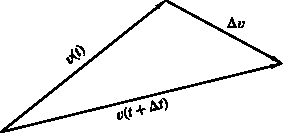
\includegraphics{figure/fig01.14}
  \caption{加速度的计算}
  \label{fig:01.14}
\end{wrapfigure}
一般如图\ref{fig:01.14}~所示。由于$a$平行于$\Delta v$,所以平均加速度的方向一
般与速度方向并不相同。瞬时加速度也类似。当加速度方向平行
于速度时,表示速度方向没有变化,但速率增加。当二者反平行
\clearpage\noindent
时,表示速度方向不变,而速率减少。当加速度既不平行也不反
平行于速度时,表示速度方向也在变化。

利用式\eqref{eqn:01.07.03},加速度矢量的分量可以表示为:
\begin{equation}\label{eqn:01.08.04}
  \vec{a}=\frac{\dif^2x\left(t\right)}{\dif t^2}\vec{i}+\frac{\dif^2y\left(t\right)}{\dif t^2}\vec{j}+\frac{\dif^2z\left(t\right)}{\dif t^2}\vec{k}
\end{equation}
加速度的三个坐标分量为:
\setlength{\mathindent}{4em}
\begin{equation}\label{eqn:01.08.05}
  a_x(t)=\frac{\dif^2x\left(t\right)}{\dif t^2},~ a_y(t)=\frac{\dif^2y\left(t\right)}{\dif t^2},~
  a_z(t)=\frac{\dif^2z\left(t\right)}{\dif t^2}
\end{equation}
\setlength{\mathindent}{6em}

$\vec{r}$,$\vec{v}$,$\vec{a}$是描写运动的物理量。我们希望用数目比较少的物
理量来描写运动。什么叫比较少?意思是这些物理量之间应是相
互独立的。所谓相互独立。是说其中任一个量不能由其他的量加
以确定。用$\vec{r}$,$\vec{v}$及$\vec{a}$三个量来描写运动是必要的,因为它们是相互
独立的。例如,在某一时刻,知道了质点的位置$\vec{r}$,并不能知道
它的速度$\vec{v}$,知道了$\vec{v}$,也并不能知道$\vec{a}$,反之亦然。人们认识到
这一点,也并不容易。在伽利略之前,并没有加速度概念。当时,
没有人认识到加速度与速度是相互独立的,所以没有认识到需要
用加速度来描写运动。

我们已讨论了位置矢量、速度和加速度。从运动学本身来考
虑,没有足够的理由说明,为什么我们应当到此为止,而不去讨
论加加速度、加加加速度……。当然,我们可以定义并计算加加
速度,即加速度的变化率,但一般说这并不代表任何具有基本物
理价值的东西。其中的原因在动力学,学过动力学后,我们将看
到,对力学的讨论几乎全部是基于位置矢量,速度和加速度这三
个量。

下面我们介绍运动的独立性这一重要概念。由式\eqref{eqn:01.05.02}、
\eqref{eqn:01.07.03}、\eqref{eqn:01.08.05}可以看到,描写一个复杂的曲线运动时,$X$方
向的坐标、速度、加速度与其他方向的坐标,速度、加速度无关。
$Y$方向和$Z$方向也有这种性质,即三个方向相互无关,这种性质被
称为运动的独立性。因此,一个复杂的曲线运动,可看成在$X$,$Y$,
$Z$三个方向上的直线运动,这三个运动同时进行,我们可以对每
一个运动进行单独的分析,好象另外两个自由度上的运动是根本
不存在一样,这样就使问题变得简单。

\example 已知一个质点作直线运动。观察到它的位置与时间
的变化如表\ref{tab:01.07}所示。用这些数据求出各时间间隔的平均速度$v$及
平均加速度$a$,并写出运动方程式。
\begin{table}[!h]
  \caption{}
  \label{tab:01.07}
  \centering
  \zihao{-5}
  \begin{tblr}{l*{9}{|X}}
    \toprule
    时~~~~间(秒)     & 0 & 1 & 2 & 3  & 4  & 5  & 6  & 7  & 8   \\
    \midrule
    {与参考点的距离 (米)} & 3 & 4 & 9 & 18 & 31 & 48 & 69 & 94 & 123 \\
    \bottomrule
  \end{tblr}
  \vspace{-0.8em}
\end{table}

\solution 因为时间间隔都是1秒,即$\Delta t=1$秒。所以从数值上有
\begin{align*}
  v & =\frac{\Delta s}{\Delta t}=\Delta s                                                            \\
  a & =\frac{\left(v_2-v_1\right)}{\Delta t}=v_2-v_1=\left(\Delta s_2\right)-\left(\Delta s_1\right)
\end{align*}
将结果列于表\ref{tab:01.08}中。
\begin{table}[!h]
  \caption{}
  \label{tab:01.08}
  \centering \zihao{-5}
  \setlength{\tabcolsep}{0em}
  \begin{tblr}{colsep=0pt,colspec={l*{17}{|X[c]}}}
    \toprule
    时~~~~间(秒) & 0 &  & 1 &  & 2 &  & 3 &  & 4 &  & 5 &  & 6 &  & 7 &  & 8 \\
    \midrule
    {与参考点的距离                                                              \\\qquad$s$~~(米)} & 3 & & 4 & & 9 & & 18 & & 31 & & 48 & & 69 & & 94 & & 123 \\
    {各秒内的位置变化                                                             \\\qquad$\Delta s$~~(米) } & & 1 & & 5 & & 9 & & 13 & & 17 & & 21 & & 25 & & 29 & \\
    {各秒内的平均速度                                                             \\\qquad$v$~~(米/秒)} & & 1 & & 5 & & 9 & & 13 & & 17 & & 21 & & 25 & & 29 & \\
    {各秒内的平均加速度                                                            \\\qquad$a$~~($\text{米/秒}^2$)} & & & 4 & & 4 & & 4 & & 4 & & 4 & & 4 & & 4 & & \\
    \bottomrule
  \end{tblr}
\end{table}
\clearpage
既然平均加速度$a$是一个常数,所以这个直线运动是匀加速
直线运动,加速度是$a=4$米/秒$^2$.对于匀加速直线运动,一般的
运动方程是:
%\vspace{-1em}
\begin{equation*}
  s=s_0+v_{0}t+\frac{1}{2}at^2 \vspace{-0.5em}
\end{equation*}
用已知数据代入,便可求出$s_0$,$v_0$,$a$。

当$t=0$时,$s=s_0=3$,所以$s_0=3$;

当$t=1$时,$4=3+v_0+\dfrac 1 2 a$,即$v_0+\dfrac 1 2 a=1$;

当$t=2$时,$9=3+2v_0+2a$,即$v_0+a=3$。

解上述两方程可得$a=4$,$v_0=-1$。所以运动方程式为:
\begin{equation*}
  s=3-t+2t^2
\end{equation*}

\example 在阴极射线管中,一束电子以$10^9$厘米/秒的速度水
平地射入平行板之间的均匀电场,电场使电子获得$10^{17}$厘米/秒\textsuperscript{2}
的向下的匀加速度。己知平行板长为2厘米。求:

\begin{wrapfigure}[8]{r}{16em}
  \centering
  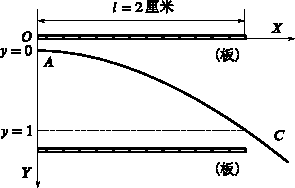
\includegraphics{figure/fig01.15}
  \caption{}
  \label{fig:01.15}
\end{wrapfigure}
(1)电子束通过平行板时的竖直方向位移$d$和经历
的时间$t$;

(2)电子束离开平行板时的速度大小和方向;

(3)在平行板内和离开板后电子束的轨迹。

\solution 选择如图\ref{fig:01.15}~所示的坐标系。

由于运动的独立性,在$x$方向是惯性运动,速度为$v_0=10^9$厘
米/秒;在$y$方向是匀加速运动,加速度为$a=10^{17}\text{厘米/秒}^2$(因为$a$
远远大于重力加速度$g$,所以不考虑重力的影响),且初速为零,
故有:

~\vspace{-1.5em}
\begin{equation*}
  \left\lbrace \begin{aligned}
    x & =v_0 t               \\
    y & =\frac{1}{2}at^2+y_0
  \end{aligned}\right.
\end{equation*}
电子通过平行板的时间为:
\begin{equation*}
  t_0=\frac{l}{v_0}=\frac{2}{10^{9}}=\num{2e-9}\text{秒}
\end{equation*}
电子通过平行板时,在竖直方向的位移为:
\begin{align*}
  d & =y_1-y_0                                      \\
    & =\frac{1}{2}at_0^2                            \\
    & =\frac{1}{2}\times 10^{17} \times \num{4e-18} \\
    & =0.2\text{厘米}
\end{align*}
电子在板中时,因为
\begin{equation*}
  v_x=v_0 \qquad v_y=at \\
\end{equation*}
\begin{align*}
  \beforetext{所以} v=\sqrt{v_x^2+v_y^2}=\sqrt{v_0^2 + a^2 t^2}
\end{align*}
速度与水平轴的夹角为:
\begin{equation*}
  \theta = \arctg\frac{v_y}{v_x} = \arctg\frac{at}{v_0}
\end{equation*}
它随时间而变。在离开板时,$t=t_0$,有
\begin{align*}
   & v \approx \num{1.02e9}\text{厘米/秒}                             \\
   & \theta = \arctg\frac{at_0}{v_0} =\arctg\frac 1 5=\ang{11;19;}
\end{align*}
在板内运动方程是:
\begin{equation*}
  \left\lbrace \begin{aligned}
    x & =v_0 t               \\
    y & =\frac{1}{2}at^2+y_0
  \end{aligned}\right.
\end{equation*}
消去$t$则得$y=\dfrac{a}{2v_0^2}x^2+y_0$,轨迹是抛物线。

离开平行板后。电子以与水平轴成\,\ang{11;19;}\,的夹角的速度
$v\approx\num{1.02e8}$厘米/秒作直线运动。

\example 设在地面附近,重力加速度是个常数$g$,且垂直指向
地面。物体的初速度为$ v_0 $。与水平方向成$ \theta $角。试讨论抛体运动
轨迹。

\discussion 我们在$ v $和铅垂线所决定的平面上来研究。按图\ref{fig:01.16}~
中的坐标,可把运动分解为$ x $方向与$ y $方向,并分别处理。$ x $方向
是惯性运动$ v_x=v_0\cos\theta $,所以有
\begin{equation*}\label{xeqn:01.08.01}
  x=\left(v_0\cos\theta\right)t \tag{1}
\end{equation*}
$ y $方向就是上抛运动,初速度为$ v_0\sin\theta$。故有
\begin{align*}
  \label{xeqn:01.08.02} & v_y=v_0\sin\theta-gt \tag{2}                          \\
  \label{xeqn:01.08.03} & y=\left(v_0\sin\theta\right)t-\frac{1}{2}gt^2 \tag{3}
\end{align*}
由\eqref{xeqn:01.08.01},\eqref{xeqn:01.08.03}消去$ t $便得抛物线形的轨迹:
\begin{equation*}\label{xeqn:01.08.04}
  y=x \operatorname{tg} \theta-\frac{g x^{2}}{2 v_{0}^{2} \cos ^{2} \theta} \tag{4}
\end{equation*}
物体达到最高点时,$ v_y=0 $,由此便得在最高点处的时间为:
\begin{equation*}
  t_{1}=\frac{v_{0} \sin \theta}{g}
\end{equation*}
相应的最大高度为,
\begin{equation*}
  \begin{aligned}
    H & =v_{0} \sin \theta\left(\frac{v_{0} \sin \theta}{g}\right)-\frac{1}{2} g\left(\frac{v_{0} \sin \theta}{g}\right)^{2} \\
      & =\frac{v^{2} \sin ^{2} \theta}{2 g}
  \end{aligned}
\end{equation*}
物体落回到与出发点同样高度时,有:
\begin{equation*}
  y=0=v_{0} t \sin \theta-\frac{1}{2} g t^{2}
\end{equation*}
\clearpage
\begin{align*}
  \beforetext{即} t_{2}=\frac{2 v_{0} \sin \theta}{g}
\end{align*}
这时的水平距离$R$叫做射程:
\begin{equation*}
  R=\left(v_{0} \cos \theta\right) t_{2}=\frac{v_{0}^{2} \sin 2 \theta}{g}
\end{equation*}
\begin{wrapfigure}[7]{r}{16.5em}
  \centering
  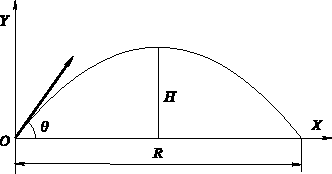
\includegraphics{figure/fig01.16}
  \caption{}
  \label{fig:01.16}
\end{wrapfigure}
因为当$\theta=\ang{45;;}$时,$\sin2\theta$
取最大值。所以,以同一速率$v_0$抛射物体,当
$\theta=\ang{45;;}$时,射程最远。
因为$\theta=\ang{90;;}$时,$\sin\theta$最
大,所以,只有当$\theta=\ang{90;;}$时,即竖直上抛,
$H$才能达到最大,其值为:
\begin{equation*}
  H_{\max }=\frac{v_{0}^{2}}{2 g}
\end{equation*}

这个题讨论的是理想情况,在实际情况中存在着空气阻力,
抛物速度愈大,阻力也愈大。空气阻力随着抛物速度的增加而逐
渐增加,在某一速度上将等于重力,这时物体将匀速下降。因而
实际上抛体的轨迹并不是理想的抛物线。
